\documentclass[a4paper]{article}

\usepackage{s}
\usepackage{amsmath,graphicx}
\usepackage{mathtools, nccmath}
\usepackage{graphicx}
\usepackage{amsmath,amssymb}
\usepackage{color,soul}
\usepackage{caption} 

\name{Gal Koaz, Gabriel Dunaevsky, Idan Kaminetsky}

\address{School of Computer Science, Ariel University, Israel}

\title{Spoken Language Recognition}

\email{koazgal@gmail.com\ gabidunaevsky10@gmail.com\ idankam98@gmail.com}

\date{April 2023}

\begin{document}

\maketitle

\section{Abstract}

In this paper, we took an existing language recognition model and tried to improve it with several methods. This model applies x-vectors to the task of spoken language recognition. This framework consists of a deep neural network that maps sequences of speech features to fixed-dimensional embeddings, called x-vectors. Long-term language characteristics are captured in the network by a temporal pooling layer that aggregates information across time. Once extracted, x-vectors utilize the same classification technology developed for i-vectors.
our work utilized datasets sourced from Common Voice, a valuable resource for multilingual speech data. We specifically focused on ten languages, carefully selected from three distinct language families: Indo-European, Semitic, and East Asian.

The main method we used to improve the existing model is changing the architecture of the TDNN layers. The first significant change is the addition of 1X1 TDNN intermediate layers between the existing layers. Another change is in the structure of the TDNN network to a funnel structure which has extensive theoretical significance by changing the number of neurons in these layers. In addition, a grid search was performed to find the optimal dilation and context size values in the TDNN layers. 

These optimal values help to find the complex patterns that represent the different languages in the audio segments. Finally, after significant training on the original data, additional training was performed for the purpose of fine-tuning the model on data with augmentations such as: changing the audio speed, adding Gaussian noise, and changing the pitch. This additional training improves the generalization ability of the model and its resistance to changes.
The purpose of the research is to present approaches to improve language recognition models and in particular, models based on the TDNN and x-vector methods. The study presents a significant improvement in relation to the existing model with the help of each of these methods and finally presents an integrated model, which contains all these changes together.

\section{Introduction}

% Introduction paragraphs subjects:
%1. Brief history and development of spoken language recognition.
%2. Introduction to spoken language recognition and its purpose.
%3. Challenges in spoken language recognition.
%4. Overview of modern language recognition systems and their reliance on i-vectors.
%5. Comparison of spoken language recognition techniques.
%6. The use of x-vectors and Vector-X technique for spoken language recognition and its potential applications.
%7. Comparison of three techniques commonly used for speaker recognition: i-vector, x-vector, and d-vector.
%8. Applications of spoken language recognition.
%9. Future of spoken language recognition.

%Idan
Idan:

The history of spoken language recognition (SLR) may be traced back to early rule-based systems, which were followed by statistical and machine learning-based approaches in the 1980s and 1990s, respectively. In recent years, advanced statistical models like GMMs paired with acoustic characteristics, as well as deep learning-based approaches such as CNNs and LSTM networks, have been successfully applied to SLR. Speech-to-text transcription, language identification in contact centers, and security are all applications of SLR. SLR systems are likely to grow more accurate and robust in the future as technology advances, allowing for increased cross-cultural communication.

%Gal
Gal:

Spoken language recognition is an exciting and vital topic that is continually evolving due to the advancement of modern technologies. Identifying the language spoken has become a vital tool for communication between diverse individuals in an era where communication crosses the borders of countries and cultures. Spoken language recognition research focuses on the development of technology and systems that allow for the automatic and more accurate identification, analysis, and understanding of spoken language. The research’s major purpose is to assist people and systems in communicating with a speaking entity in a language they do not understand, as well as to increase communication and efficiency between people and systems. The creation of advanced algorithms and models, such as the recognition of the manner of speaking and auxiliary effects in speech, as well as the production of databases and their usage to run more accurate language recognition systems, may be included in the research techniques.

%Idan
Idan:

Although spoken language recognition has made great progress over the years, there are still several hurdles that must be overcome in order to produce accurate and dependable findings. Background noise is one of the most serious issues, as it can considerably reduce the accuracy of spoken language recognition systems. Noise can come from a multitude of sources, including traffic, wind, and other external variables, as well as other speakers in the same room or nearby. Variations in dialects and accents are another problem. People frequently talk with varied accents and dialects, even within the same language, making it challenging for voice recognition algorithms to reliably identify the spoken language. This is especially difficult in countries with a significant degree of linguistic diversity, such as India, where different regions have their own distinct dialects and accents. 

Idan:

Another issue is a lack of training data. To learn and increase their accuracy over time, speech recognition algorithms rely substantially on training data. Obtaining huge volumes of high-quality training data, on the other hand, might be problematic, especially for languages with fewer speakers or dialects that are not commonly spoken. As a result, models may be under-trained, resulting in poor accuracy and reliability. Furthermore, spoken language recognition systems may have difficulty identifying spoken language in real-time, especially when dealing with spontaneous speech, such as in genuine conversation. The necessity for fast and efficient algorithms that can handle massive amounts of data in real-time makes real-time processing difficult. Overall, these difficulties in spoken language recognition underscore the importance of ongoing research and development in this sector in order to enhance the accuracy and reliability of these systems. To address these problems and increase the performance of spoken language recognition systems, further technological breakthroughs, such as improved algorithms and data collection methods, will be required.

%Gal
Gal:

Speaker embedding is a critical problem in Spoken Language Recognition (SLR) that includes extracting compact and discriminative representations from voice data. The most prevalent speaker embedding techniques are x-vector, i-vector, and d-vector. The x-vector approach uses a deep neural network (DNN) to extract a variable-length speaker embedding from a speech signal. The DNN is trained on a large amount of speaker-labeled data and is typically composed of convolutional and recurrent layers to capture both short-term and long-term information from the speech signal. The resulting x-vector is a low-dimensional representation that can be used for speaker verification, speaker identification, and language identification tasks. 


Gal:

The i-vector approach uses a factor analysis model to extract a fixed-length speaker embedding from a speech signal. The i-vector is typically extracted from a low-dimensional representation of the speech signal using a probabilistic model called a Gaussian mixture model-universal background model (GMM-UBM), for more information \cite{morrison2011comparison}. The i-vector captures the speaker-specific information from the speech signal and has been widely used in speaker verification tasks. However, it is less commonly used in speaker identification and language identification tasks due to its fixed-length representation. The d-vector approach is similar to the x-vector approach but is trained with a larger amount of data and a longer sequence of speech signals. The d-vector is typically extracted from a deep neural network that is trained on large-scale speaker-labeled data, and it aims to capture the speaker-specific information from the entire speech segment. The resulting d-vector is a low-dimensional representation that can be used for various SLR tasks, including speaker verification, speaker identification, and language identification. Compared to the i-vector, the d-vector is more robust to varying speech conditions and has shown promising results in various SLR applications.


%Gal
Gal:

The majority of modern language recognition systems rely on i-vectors
\cite{najim2011front}. The conventional method consists of a universal background model (UBM) and a huge projection matrix T that are trained to maximize the likelihood of the training data. The projection converts the (UBM) high-dimensional statistics into a low-dimensional form known as an i-vector. I-vectors are typically categorized after extraction using Gaussian models, logistic regression, or cosine scoring. Deep neural networks (DNN) trained as acoustic models for automated speech recognition (ASR) are used in cutting-edge i-vector systems. This is frequently achieved in one of two ways: either the ASR DNN posteriors replace those from a Gaussian mixture model (GMM), or the i-vector system is trained using bottleneck characteristics extracted from the DNN \cite{matejk2014neural,richardson2015neural}.

%Idan
Idan:

The various techniques for spoken language recognition (SLR) are categorized into two types: feature-based and model-based. Model-based strategies develop models of language-specific characteristics, whereas feature-based methods extract acoustic features. Some of the most often used SLR techniques are the Gaussian Mixture Model (GMM), the Hidden Markov Model (HMM), the Support Vector Machine (SVM), Neural Networks (NN), Convolutional Neural Network (CNN), and Long Short-Term Memory (LSTM). Each technique has advantages and disadvantages, and the technique used is determined by the individual application and available training data. In addition, neural network-based algorithms, such as CNNs and LSTMs, are excellent for dealing with complex feature spaces and temporal fluctuations in voice signals, but they require a significant amount of training.

%Gal
Gal:

In this article, we will look at the technologies used to recognize spoken language and the technical and practical issues that arise as a result of this process. We use x-vectors to perform spoken language recognition. To evaluate and represent data in vector space, the Vector-X technique is utilized. In the case of spoken language identification, Vector-X may be beneficial as a tool for studying and modeling speech. When using Vector-X for spoken language identification, the main job is to represent the voice as a vector in vector space. This vector represents the entire speech, including the words used, the grammatical structure of the speech (e.g., tenses, degrees, and so on), and any specific speech processing (e.g., voice pressure, tone, and so on). This data can be utilized as consistent information for machine learning models for recognizing and classifying spoken language by comparing the vector encoding of the voice to applicable language models. Furthermore, Vector-X may be utilized to distinguish between speaker goals, identify the melody used in the speech, and grasp the speaker’s tone. To read more about X-vectors \cite{raj2019probing}.

\begin{table}[ht]
\centering
\caption{Comparison of i-vector, x-vector, and d-vector}
\label{tab:vector-comparison}
\resizebox{0.5\textwidth}{!}{%
\begin{tabular}{|c|c|c|c|}
\hline
\textbf{Technique} & \textbf{i-vector} & \textbf{x-vector} & \textbf{d-vector} \\
\hline
Representation & Low-dim. & High-dim. & High-dim. \\
\hline
Modeling & Generative & Discriminative & Hybrid \\
\hline
Training & Supervised & Supervised & Sup./Unsup. \\
\hline
Architecture & GMM-UBM & CNN & LSTM \\
\hline
\end{tabular}%
}
\end{table}

%Gal
Gal:

Table 1 provides a comparison of three techniques commonly used for speaker recognition: i-vector, x-vector, and d-vector. It highlights differences in their representation, modeling approach, training, and architecture. The i-vector is a low-dimensional technique with a generative modeling approach and requires supervised training using a GMM-UBM architecture. The x-vector is a high-dimensional technique with a discriminative modeling approach, requiring supervised training using a CNN architecture. The d-vector is a hybrid approach with high-dimensional representation, requiring both supervised and unsupervised training using an LSTM architecture.


%Idan
Idan:

Spoken language recognition has numerous applications in security, language acquisition, speech treatment, customer service, and virtual assistants. It can be used in security systems to detect unauthorized access and identify suspects in forensic investigations. It can provide feedback on pronunciation and intonation to language learners and construct tailored language learning programs. It can diagnose speech abnormalities and give tailored therapy in speech therapy. Spoken language recognition can also be used in customer service and virtual assistants to improve communication and more precisely understand voice commands.

%Idan
Idan:

The use of natural language processing and machine learning methods to improve the accuracy of language recognition systems is part of the future of spoken language recognition. There is also a priority on developing systems that can understand emotions and intent in spoken language, which could be valuable in customer service and healthcare applications. Deep learning techniques, for example, are likely to play a key role in enhancing the accuracy of language recognition systems. The advancement of spoken language recognition technology has enormous implications for cross-cultural communication, and it has the potential to play a critical role in breaking down language barriers and creating greater understanding and collaboration among individuals from various backgrounds.



\section{Related Work}
%Gabi
Gabi:

There is a lot of information and studies about this subject.
In \cite{zazo2016language}, a different approach has been taken.
They presented an LSTM RNN system running on limited computational resources (a single GPU) that outperforms a reference i-vector system on a subset of the NIST Language Recognition Evaluation (8 target languages, 3s task). In addition they extended previous
experiments modeling unseen languages, They also analyze the effect of even more limited test data and they proved that with as little as 0.5s an accuracy of over 50\% can be achieved they also claiming that LSTM RNN based
approaches using open source implementations outperform the standard i-vector based approach when dealing with short test durations with an improvement of $\sim$26\% in terms of
Equal Error Rate with respect to the reference i-vector based system.

%Gabi
Gabi:

another work by \cite{alan2014multiclass}, trained i-vectors with Multiclass Discriminative.They showed an approach where a Gaussian i-vector classifier is trained using Maximum Mutual Information (MMI) to directly optimize the multiclass calibration criterion so that no separate back-end is needed. Results on the NIST LRE11 standard evaluation task confirm that high performance and calibration are maintained with this new single-stage approach.In addition, the system is
extended to the open set task using the additive Gaussian
noise model, and this is also discriminatively trained to
improve performance.

%Gabi
Gabi:

A different work by \cite{shubham2018multilingual}, also took a different approach. They present a single sequence-to-sequence automatic speech recognition (ASR) model trained on 9 different Indian languages, which have very little overlap in their scripts. They took a union of language-specific grapheme sets and train a grapheme-based sequence-to-sequence model jointly on data from all languages. They found that this model, which is not explicitly given any information about language identity, improves recognition performance by 21\% relative compared to analogous sequence-to-sequence models trained on each language individually. They also modified the model to accept a language identifier as an additional input feature and improved performance by an additional 7\% relative and eliminate confusion between different languages.

%Gabi
Gabi:

In \cite{daniel2016stacked}, they tried a different way. They introduce a stacked architecture that uses a time delay neural network (TDNN) to model long-term patterns for spoken language identification.The first component of the architecture is a feed-forward neural network with a bottleneck
layer that is trained to classify context-dependent phone states (senones). The second component is a TDNN that takes the
output of the bottleneck, concatenated over a long time span,
and produces a posterior probability over the set of languages. The proposed system outperforms a state-of-the-art shifted delta cepstra i-vector system and provides complementary information to fuse with the new generation of bottleneck-based i-vector systems that model short-term dependencies. The proposed system provides a relative gain of 27\% in identification accuracy.

%Gabi
Gabi:

In \cite{alan2018language}, they were using a Deep neural networks (DNN) and bottleneck joint i-vector systems.they did it by using discriminative Gaussian classifier combined with naive fusion used all of the development data for system  design rather than holding some out for separate back-end training. They replaced i-vectors with more powerful x-vectors to further improve language recognition accuracy. They were able to achieve the  JHU HLTCOE LRE17 language
recognition system which gave them very good results.

%Gabi
Gabi:

In \cite{david2018spoken}. They apply x-vectors to the task of spoken language recognition and deep
neural network (DNN). They found that long-term language characteristics are captured in the network by a temporal pooling layer that aggregates information
across time. Once extracted, x-vectors utilize the same
classification technology developed for i-vectors. Finally they found that the best-performing system uses multilingual bottleneck features, data augmentation, and a discriminative Gaussian classifier.

%Gabi
Gabi:

In \cite{yun2014application}. They propose  two novel frontends for robust language identification (LID) using a convolutional neural network (CNN) trained for automatic speech recognition (ASR).
The results that they got are complementary and give significant gains of up to 20\% relative to the best single system when combined.

Gabi:

In \cite{david2011language}, they showed a way using iVectors Space.
here they recognize language in the iVector space, they e experiment with three different linear classifiers which one based on a generative model (SVM), where classes are modeled by Gaussian distributions with shared covariance matrix, and two discriminative classifiers, namely linear Support Vector Machine and
Logistic Regression. Their dataset contain 23 target languages, and files of 3, 10 and 30 s. The results are shown in terms of Cavg ×100 defined in the NIST LRE 2009 Evaluation Plan \cite{NISTLRE2009EvaluationPlan}.

Gabi:

In \cite{Jorgen2020VOXLINGUA107}, they investigated the use of automatically collected web audio data. They generate semirandom search phrases from language-specific Wikipedia data that
are then used to retrieve videos from YouTube for 107 languages. Speech activity detection and speaker diarization are used to extract
segments from the videos that contain speech. The size of the resulting training set (VoxLingua107) is 6628 hours (62 hours per language on the average) and it is accompanied by an evaluation set of 1609 verified utterances. Another thing that they are doing is a post-filtering to remove segments from the database that are likely not in the given language which is increasing the proportion of correctly labeled segments to 98\%, based on crowd-sourced verification.

Gabi:

In \cite{Gundeep2021Spoken}, They was working with audio clips by unknown speaker, regardless of gender, manner of speaking, and distinct age speaker. The model uses audio files and converts those files into spectrogram images. The model applies the convolutional neural network (CNN) to bring out main attributes or features to detect output easily. The main objective is to detect languages out of 25 languages such as English, French, Spanish, and German. To this expirament they was using a data set from Kaggle. These audio files are comprised of utterances, each of them spanning over a fixed duration of 10 seconds. The whole dataset is split into training and test sets. Preparatory results give an overall accuracy of 98\%. Extensive and accurate testing show an overall accuracy of 88\%.

\section{Datasets}

% For this work we were using Datasets that we found in Common Voice. We chose to work with ten different languages from three different types of languages :

% 1.Indo Europeans languages.

% 2.Semitic languages.

% 3.East Asian languages.

% We chose specifically this types of languages because of the diversity between this languages, there for in the Indo Europeans languages we chose : Spanish, French, Italian and Russian. The Semitic languages includes : Arabic, Hausa and Farsi. From the East Asian languages we took: Chinese, Japanese, Thai. The impotence of recognition among this languages is big because there are many people that speaks this languages and around the world that are not speaking English which considers an international language.
Gabi:

In the field of speech recognition, the ability to accurately transcribe and understand diverse languages is of utmost importance. To address this challenge, our work utilized datasets sourced from Common Voice, a valuable resource for multilingual speech data. We specifically focused on ten languages, carefully selected from three distinct language families: Indo-European, Semitic, and East Asian. This article aims to shed light on the significance of recognizing and supporting speech recognition in these languages, considering the substantial number of non-English speakers worldwide. We believe that with these languages Our work aimed to contribute to the development of multilingual speech recognition systems. Such systems have the potential to bridge language barriers, empower non-English speakers, and foster inclusivity on a global scale.\newline


Gabi:

1. Indo-European Languages:

Among the Indo-European language family, we chose to include Spanish, French, Italian, and Russian in our study. These languages were selected for their remarkable diversity and widespread usage across multiple continents. By incorporating languages from different regions, we aimed to capture the richness and variation present within this language family. Now we will present some information about each language that we were using in the Indo-European Languages before the pre-process:

1. Spanish - in the Spanish language there is 24 Recorded hours and 11 Validated hours. The number of different speakers in the language are 207 speakers.

2. French - in the French language there is 12 Recorded hours and 15 Validated hours. The number of different speakers in the language are 298 speakers.

3. Italian - in the Italian language there is 4 Recorded hours and 4 Validated hours. The number of different speakers in the language are 49 speakers.

4. Russian - in the French language there is 8 Recorded hours and 5 Validated hours. The number of different speakers in the language are 103 speakers.\newline

Gabi:

2. Semitic Languages:

In our research, we recognized the importance of Semitic languages, which have historical and cultural significance in various parts of the world. To represent this language family, we focused on Arabic, Hausa, and Farsi. These languages are spoken by millions of people globally and play a vital role in their respective communities. By including Semitic languages in our study, we aimed to address the specific challenges and intricacies associated with their speech recognition. Here is some statistics about each language that we were using in the Semitic Languages before the pre-process:

1. Arabic - in the Arabic language there is 2 Recorded hours and 1 Validated hours. The number of different speakers in the language are 77 speakers.

2. Hausa - in the Hausa language there is 13 Recorded hours and 4 Validated hours. The number of different speakers in the language are 39 speakers.

3. Farsi - in the Farsi language there is 2 Recorded hours and 4 Validated hours. The number of different speakers in the language are 37 speakers.\newline

Gabi:

3. East Asian Languages:

The third group we explored consisted of East Asian languages. Chinese, Japanese, and Thai were selected as representatives of this diverse and vibrant language family. East Asian languages possess unique phonetic structures and tonal characteristics, making them intriguing subjects for speech recognition research. Given the sizable populations that speak these languages, their accurate recognition holds great significance for enabling effective communication and access to technology for non-English speakers. We will present some knowledge about each language that we were using in the East Asian Languages before the pre-process:

1. Chinese - in the Chinese language there is 5 Recorded hours and 95 Validated hours. The number of different speakers in the language are 189 speakers.

2. Japanese - in the Japanese language there is 4 Recorded hours and 3 Validated hours. The number of different speakers in the language are 36 speakers.

3. Thai - in the Thai language there is 7 Recorded hours and 5 Validated hours. The number of different speakers in the language are 77 speakers.\newline

Gabi:

\begin{table}[ht]
\centering
\caption{Languages and sub-languages}
\label{tab:Languages}
\resizebox{0.5\textwidth}{!}{%
\begin{tabular}{|c|c|}
\hline
\textbf{Languages} & \textbf{sub-languages} \\
\hline
Indo-European & Spanish,French,Italian,Russian. \\
\hline
 Semitic & Arabic,Hausa,Farsi. \\
\hline
 East Asian & Chinese,Japanese,Thai.\\
\hline
\end{tabular}%
}
\end{table}

* A quick note about the data is that every data contains male and female as speakers, the ages of the speakers are between teenagers to old and for each language there are several dialects inside the segments. Unfortunately we were not able to find some information about the distribution for each language on this statistics.\newline

Another thing that is important to mention is the differences between Recorded hours and Validated hours in Common Voice dataset.

- Recorded hours refer to the total amount of audio data that has been contributed to the Common Voice project. It represents the cumulative duration of all the voice recordings that users have submitted.

- Validated hours, on the other hand, represent the subset of recorded hours that have been manually reviewed and verified by the Common Voice community. The validation process involves volunteers listening to and evaluating the contributed recordings to ensure they meet certain quality criteria, such as clarity, naturalness, and adherence to the specified prompts. Validated hours reflect the portion of recorded data that has been approved and deemed suitable for use in training machine learning models.

Understanding languages, not speakers it's crucial for the model to learn the linguistic content rather than the specific characteristics of individual speakers. This is due to several reasons:

1. Generalization: The goal of models in speech recognition or language identification is to understand the spoken content, regardless of who the speaker is. If the model learns to recognize specific speakers instead of the language, it may fail to generalize to new speakers. This could severely limit the model's utility in real-world applications, as it would only work well for speakers it has been trained on.

2. Variation in speech characteristics: Each individual speaker has unique speech characteristics, such as pitch, speed, accent, etc. If a model is trained on data from a limited number of speakers, it might become biased toward those specific speakers' characteristics. To ensure the model works well with a wide range of speakers, it is important to include a diverse set of speakers in the training data.

3. Privacy considerations: In many applications, the identity of the speaker is sensitive information. Models that focus on understanding languages rather than identifying speakers are more privacy-friendly, as they don't need to store or learn from personal voice characteristics.

4. Efficiency and scalability: Learning languages rather than speakers is generally a more scalable approach. There are potentially billions of different speakers, but only a few thousand languages. It would be much more efficient to build models that understand languages rather than trying to handle each individual speaker separately.

5. Addressing data imbalance: In most datasets, the number of utterances per speaker is often imbalanced, with some speakers being over-represented and others under-represented. If a model learns to recognize speakers, it may become biased towards speakers with more data. On the other hand, focusing on languages allows the model to learn more generalized, language-specific features.

Gabi:

As part of the research, we decided to make a pre-process on the dataset that we took from common voice. First of all Data preprocessing is an important step in any machine learning or data analytics project because raw data collected from various sources frequently contains noise, outliers, missing values, or is in an unusable format. The goal of preprocessing is to transform this raw data into a clean, understandable, and efficient format suitable for machine learning algorithms. It improves the quality and reliability of the data, reduces complexity, and can improve the accuracy and efficiency of the subsequent analysis or prediction. Without preprocessing, machine learning models may be built on inaccurate or irrelevant data, resulting in misleading or incorrect results. In our article, several steps were performed:

\subsection{Balanced data}

Idan:

The first thing that was done is to take the same amount of data from each language. We chose the minimum number of voice segments that we had among these 10 languages, which was 994 segments so totally we are working with 9940 voice segments. The impotence of working with balanced data is very big and this is several reasons that explain this:\newline
%% to check

1. Avoiding Bias: Imbalanced data can introduce bias in predictive models. When the dataset is skewed towards one class, the model can become overly sensitive to the majority class and may struggle to accurately predict the minority class. This can lead to poor performance and skewed results.\newline

2. Accurate Representation: Balanced data ensures that each class is represented equally, allowing the model to learn from a diverse range of examples. It helps in capturing the true distribution of the data and prevents the model from making assumptions based on an imbalanced representation.\newline

3. Reliable Evaluation: Working with balanced data allows for a more reliable evaluation of model performance. When evaluating the model on imbalanced data, metrics like accuracy can be misleading. For instance, if 95\% of the data belongs to the majority class, a model that predicts all instances as the majority class will have high accuracy, even though it fails to classify the minority class correctly. Balanced data enables more accurate assessment of metrics like precision, recall, and F1-score.\newline

4. Improved Generalization: Models trained on imbalanced data may struggle to generalize well to new, unseen data. Balanced datasets help models to learn more robust and representative patterns, which can improve their ability to make accurate predictions on unseen examples.\newline

5. Better Decision Making: In domains where the cost of misclassification is significant, such as healthcare or fraud detection, working with balanced data becomes crucial. A model trained on imbalanced data might make incorrect predictions that have severe consequences. By balancing the data, the model can make more informed decisions across all classes.

After The Creation of 994 segments to each language we decided to divide the data to 3 parts which are:

-Train

-Test

-Validation

Gal:

We decided to split the data as follows (Train - 70\%, Validation - 20\%, Test - 10\%).
Splitting the data into training, testing, and validation sets is a crucial step in the development and evaluation of machine learning models. Here are the main reasons why data splitting is important:

* Model Training: The training set is used to train the machine learning model. It contains labeled data that the model uses to learn patterns and relationships between input features and their corresponding outputs. By exposing the model to a diverse range of examples during training, it can better generalize and make accurate predictions on unseen data.

Gal:

* Model Evaluation: The testing set is used to evaluate the performance of the trained model. It contains labeled data that the model has not seen during training. By evaluating the model on this independent dataset, we can assess its ability to generalize and make accurate predictions on new, unseen data. This helps us understand how well the model is likely to perform in real-world scenarios.

* Hyperparameter Tuning: Hyperparameters are configuration settings that are not learned from the data but are set prior to training. These include parameters like learning rate, batch size, regularization strength, etc. The validation set is used to tune and optimize these hyperparameters. Multiple models with different hyperparameter settings can be trained and evaluated on the validation set to select the best-performing model. This helps prevent overfitting and improves the generalization ability of the model.

* Preventing Data Leakage: Splitting the data into separate sets helps prevent data leakage, which can lead to biased and overly optimistic performance estimates. Data leakage occurs when information from the test or validation sets unintentionally leaks into the training process. By keeping these sets isolated, we can obtain unbiased estimates of the model's performance on new, unseen data.

* Generalization Assessment: The testing set provides an unbiased estimate of the model's performance on new, unseen data. It helps determine whether the model has learned meaningful patterns and can generalize well beyond the training data. By evaluating the model's performance on the testing set, we can make informed decisions about deploying the model in real-world applications.

Overall, data splitting into training, testing, and validation sets is essential for building robust and reliable machine learning models. It helps in training the model, evaluating its performance, tuning hyperparameters, preventing data leakage, and assessing generalization ability.

\subsection{Convert files}

Gal:

The second thing that was done is to convert the mp3 files that we were receiving from Common Voice to wav files, There are reasons to convert audio files from MP3 to WAV format. The following are the primary reasons:

1. Lossless vs. Lossy Compression: MP3 is a lossy format, which means that it compresses data by deleting sections of the audio that are judged less detectable to human hearing. This can lead to a loss of audio fidelity as well as potentially important data for research. WAV, on the other hand, is a lossless format that preserves all of the data in the audio file. When performing an audio analysis, it is critical to keep all data because the rejected parts of lossy compression may contain essential information.

2. Uncompressed Data: Because WAV files include raw and uncompressed data, they are easier to manipulate and analyze immediately. WAV files' uncompressed data can be easily read into data structures like arrays for additional processing, making it easier to work with in programming environments.

3. Sampling Rate Consistency: Consistent sample rates are critical when studying sound. Because MP3 compression might cause different sampling rates across the file, feature extraction may be uneven. WAV files, on the other hand, keep a constant sample rate throughout the file.

4. Compatibility with Libraries: Some audio analysis libraries function better with WAV files than others. Python tools for audio and music analysis, such as Scipy and Librosa, may, for example, handle WAV files more directly and effectively than MP3 files.

\subsection{Cleaning data}

Gal:

The third thing that was done in the pre-process that we did is to "clean" all the "dead" parts for each segment that we are working with, in any data analysis or machine learning project, the quality and cleanliness of the data used play a vital role in determining the accuracy and reliability of the results.
When saying "dead" parts we mean to the portions of data within a particular segment that has no voice or the voice is very low proportional to the thresh hold that we determined which means these segments are irrelevant.
here are some advantages to "clean the data:\newline

1. Enhanced Accuracy: Removing "dead" parts eliminates outdated or irrelevant data, ensuring that the analysis is focused on the most current and meaningful information. This helps in reducing noise and unnecessary complexity in the dataset.\newline

2. Improved Data Integrity: By cleaning out redundant or invalid data, the overall integrity and consistency of the dataset are improved. This increases the reliability of subsequent analyses and models built upon the cleaned data.\newline

3. Unbiased Analysis: By removing "dead" parts, we reduce the risk of bias that can arise from including irrelevant or outdated data. A clean dataset ensures that the analysis is based on accurate and representative information, leading to more reliable insights and decisions.


\subsection{Data augmentation}

Gal:

The fourth thing that was done with the dataset is to generate another three different types to get three different augmentations. The extra three augmentations that we choose are:\newline


1. Speed: Modifying the speed of audio clips can simulate the variation in speech rate among different speakers. By accelerating or decelerating speech signals, we can generate new training instances and help the model become invariant to the rate of speech. It may improve the model's ability to understand fast or slow speakers.\newline

2. Pitch: Pitch perturbation is a way to mimic the natural variation in the pitch of human voices. Shifting the pitch of the audio signal can also help make the model robust to different speaker characteristics. A model trained with pitch-augmented data might better handle audio from speakers with unusually high or low pitches.\newline

3. Noise: Adding different types of noise to your audio data is a common way to simulate real-world conditions, where clean, noise-free audio is rarely available. This can help improve the model's performance in noisy conditions. Different types of noise (white noise, pink noise, environmental noise) could be used based on the application.\newline


There are several reasons why data augmentation is important to us and as a result, we have implemented these methods in our process\newline

1. Improving model performance: Data augmentation techniques create variations of the existing data, helping the model learn and generalize better. This can lead to improved performance on unseen data and enhance the robustness of the model.\newline

2. Mitigating overfitting: Overfitting is a common problem in machine learning where a model learns the training data too well and performs poorly on unseen data. By increasing the diversity and size of the training data through augmentation, the model can be prevented from memorizing the training examples and instead, learn more general patterns.\newline

3. Addressing class imbalance: In many real-world scenarios, the distribution of classes in the data is imbalanced, which can bias the model towards the majority class. Augmentation can be used to create more instances of the minority class(es), balancing the class distribution and helping the model to learn more representative features of each class.\newline

4. Simulating real-world conditions: Especially in fields like image and audio processing, data augmentation can simulate different real-world conditions that were not present in the original dataset, such as different lighting conditions in images or background noise in the audio.\newline

\section{Framework}

\subsection{Loss Function}

Gabi:

In the new model and the baseline model as well Cross Entropy Function Loss is used.
A presentation of a simple cross-entropy function:

$$-{(y\log(p) + (1 - y)\log(1 - p))}$$

Where:

- p is the predicted probability, and

- y is the indicator (0 or 1 in the case of binary classification)
\newline

Basically, Cross entropy loss measures the difference between the discovered probability distribution of a machine learning classification model and the predicted distribution.

in more detail the cross-entropy between two probability distributions 
p and q over the same underlying set of events measures the average number of bits needed to identify an event drawn from the set if a coding scheme used for the set is optimized for an estimated probability distribution 
q, rather than the true distribution p.

To read more on the Cross-Entropy Function Loss, \cite{chen2012cross}.


\subsection{Introduction to Baseline Model}

Gal:

\begin{figure}[htp]
    \centering
    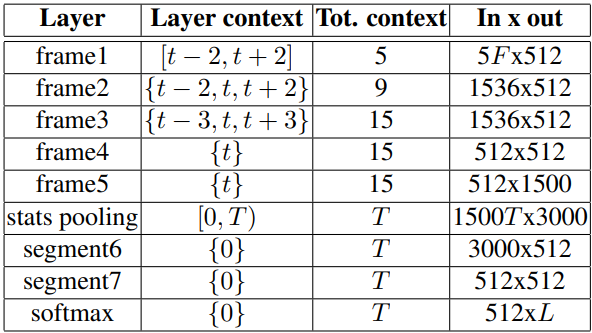
\includegraphics[width=8.5cm]{table.png}
    \caption{Architecture Source Model}
\end{figure}

The x-vector DNN architecture is the most common. Before the nonlinearity, x-vectors are extracted at layer segment 6. F-dimensional characteristics can be accepted by the input layer.
The softmax layer's L denotes the number of training languages.

Gal:

The DNN configuration is outlined in Table 1. The
input to the DNN is a sequence of T speech frames.
The first five layers process the data on a frame-by-frame basis, with a limited temporal context centered on the current frame t.
The input layer, frame1, for example, splices together the F-dimensional features at frames t 2, t 1, t, t + 1, and t + 2, giving it a total temporal context of 5 frames. The following layer's input, frame2, is the spliced output of frame1 at t 2, t, and t + 2. This layer extends the temporal context produced by the previous layer, giving frame2 a total context of 9 frames. This technique is repeated in the subsequent layers, resulting in frame 5 viewing a total context of 15 frames.

Idan:

The statistics pooling layer collects data across time dimensions, allowing the following layers to function on the full segment. A sequence of T 1500-dimensional vectors from the previous layer, the frame5, is fed into the pooling layer. The result is the mean and standard deviation of the input (each vector has 1500 dimensions). These statistics are concatenated (to form a 3000-dimensional vector) and sent via the segment-level levels before reaching the softmax output layer.
The nonlinearities are represented using rectified linear units (ReLUs). Section 6 networks have between 4.2 and 4.6 million parameters.

Idan:

\subsection{The New Model}

\begin{table}[ht]
\centering
\caption{Architecture our Model}
\label{tab:model}
\resizebox{0.5\textwidth}{!}{%
\begin{tabular}{|c|c|c|c|c|}
\hline
\textbf{Layer} & \textbf{Layer context} & \textbf{Tot. context}  & \textbf{Tot. width of context} & \textbf{In x out}\\
\hline
frame 1 & \{t-2,t+2\}& 3 & 5 & 3Fx1280 \\
\hline
frame 2 & \{t\} & 3 & 5 & 1280x1280 \\
\hline
frame 3 & \{t-4,t-2,t,t+2,t+4\} & 7 & 9 & 8960x1024 \\
\hline
frame 4 & \{t\} & 7 & 9 & 1024x1024 \\
\hline
frame 5 & \{t-1,t+1\} & 9 & 11 & 9216x768 \\
\hline
frame 6 & \{t\} & 9 & 11 & 768x512 \\
\hline
frame 7 & \{t\} & 9 & 11 & 512x256 \\
\hline
stats pooling & [0,T) & T & T & 256Tx512 \\
\hline
segment 8 & \{0\} & T & T & 512x512 \\
\hline
segment 9 & \{0\} & T & T & 512x512 \\
\hline
softmax & \{0\} & T & T & 512xL \\
\hline
\end{tabular}%
}
\end{table}

The table presented above shows the new structure of the integrated Model in this research. A 2 new layers were added (layer 2 and layer 4) these 2 layers were added as an intermediate layers and not part of the funnel structure. The rest layers changed to be in the structure of a funnel.\newline 

\begin{figure}[htp]
    \centering
    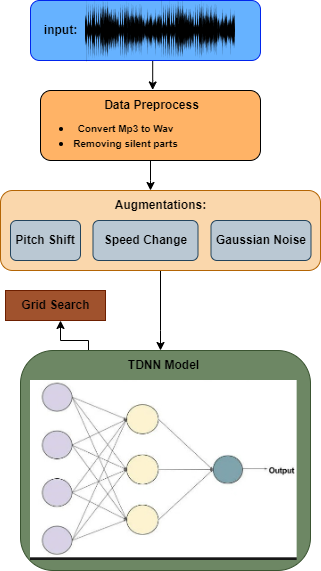
\includegraphics[width=5.5cm]{Untitled Diagram.drawio (3).png}
    \caption{Structure of the network}
\end{figure}


Idan:

In our method, we chose to work on the BASELINE MODEL and change its architecture and hyperparameters in several ways to improve the model's generalizability and its results. We ran the changes we made separately on the baseline model to see the significance of each of the changes. In the article, we will present 3 key changes that significantly improved the results of the model: 

1. Grid Search on the 'context size' and 'dilation' hyperparameters in the TDNN layers. 

2. Changing the number of neurons in the TDNN layers from a fixed number (512) to a funnel shape. 

3. Adding intermediate layers for further processing of the frames and context.

In the following sections, we will present each of these changes in detail. We will include a general explanation of each topic, the theoretical meaning of these changes, important details about the actual implementation and finally, we will present the results. In the end, we created an integrated model which contains these three improvements. The results of this model will be presented later.


% In this research several things were done that will be elaborated right now. This research is based on a previous research \cite{david2018spoken}. A general things that were changed from the  previous research are to change the number of epochs (from 30 to 100) and the batch number (from 10 to 100). By increasing the number of epochs we are training the model more which are giving more "knowledge" and power to our model on one hand, but on the other hand there is a danger of over fitting, so it's have to done carefully. By increasing the natch size we can find some advantages, for example: 

% 1. Faster computation

% 2. Efficient memory utilization

% 3. More stable gradient estimates

% 4. Improved generalization

% 5. Noise reduction

% But as well as increasing the epochs number it has to be done carefully. Larger batch sizes can require more memory, which may limit the model's scalability on certain hardware configurations. Additionally, extremely large batch sizes may lead to slower convergence or get stuck in suboptimal solutions. To read more about the importance of the batch size you can read here \cite{keskar2016large}.

\subsection{Grid Search for Context Size and Dilation Hyper-parameters}

Idan:

In TDNN (Temporal Convolutional Neural Network) layers, the concepts of context size and dilation play crucial roles in capturing temporal dependencies and modeling sequential data.

The context size in a TDNN layer refers to the number of adjacent frames or time steps considered during the convolution operation. It determines the range of temporal information that the layer can capture. A larger context size allows the layer to incorporate a broader temporal context, whereas a smaller context size focuses on local temporal relationships. By considering a wider context, TDNN layers can capture longer-range dependencies and learn higher-level temporal patterns in the data. This can be particularly useful in tasks where understanding longer-term context is important, such as speech recognition or natural language processing. On the other hand, smaller context sizes are more suitable for capturing fine-grained details and immediate temporal relationships. The choice of an appropriate context size depends on the specific characteristics of the data and the task at hand. It requires balancing the need to capture relevant temporal dependencies while avoiding excessive computational complexity or overfitting.

Idan:

Dilation refers to the spacing between the input frames or time steps that the TDNN layer considers during the convolution operation. It controls the skip or gap between the frames and influences the receptive field of the layer. In TDNN layers, a dilation of 1 means that there is no skip or gap between the input frames. Each frame is considered sequentially during the convolution. A dilation greater than 1 introduces skips or gaps between the frames, allowing the layer to capture non-adjacent temporal relationships and capture information at larger time scales. By using dilation, TDNN layers can capture temporal dependencies that span a larger range without significantly increasing the number of parameters or computational complexity. This is particularly useful for modeling long-range dependencies and capturing global temporal patterns in the data. The choice of dilation value depends on the specific requirements of the task and the desired balance between capturing local and global temporal relationships. Smaller dilation values (e.g., 1) are suitable for capturing fine-grained local patterns, while larger dilation values allow for modeling longer-range dependencies.

In summary, the context size and dilation in TDNN layers are essential parameters for modeling sequential data. The context size determines the range of temporal information considered, while dilation controls the skip or gap between frames and influences the receptive field. Choosing appropriate values for context size and dilation is crucial for capturing relevant temporal dependencies, modeling different temporal scales, and effectively learning from sequential data. 

Grid search is a good way to find optimal values for dilation and context size. Grid search is a systematic and exhaustive search method that can be used to find optimal values for dilation and context size in TDNN layers. It involves defining a grid of possible values for each hyperparameter and evaluating the model's performance for all possible combinations of these values.

Idan:

Grid search is a technique used for hyperparameter optimization in machine learning. It involves defining a grid of hyperparameter values to be searched exhaustively. The grid search algorithm then trains and evaluates the model for each combination of hyperparameters in the grid and selects the one that performs the best.
the steps involved in grid search:

1. Define the hyperparameters to be tuned: Identify the hyperparameters in your model that you want to optimize. In our project, those are context size and dilation in the 3 first TDNN layers.

2. Define the grid: Specify the set of possible values for each hyperparameter. context size values are [2, 3, 5, 7] and dilation values are [1, 2, 3].

3. Generate combinations: Create all possible combinations of hyperparameters from the defined grids.

4. Training and evaluation: For each combination of hyperparameters, train the model using the training dataset and evaluate its performance using a validation set. This involves fitting the model, making predictions, and computing a performance metric.

5. Select the best combination: Compare the performance of models trained with different hyperparameter combinations and select the one with the best performance metric. This is typically done by choosing the hyperparameters that maximize the metric or minimize a loss function.

As mentioned above, grid search exhaustively explores all possible combinations of hyperparameters, which can be computationally expensive for large hyperparameter spaces. However, it ensures a thorough search and can help in finding the optimal set of hyperparameters for your model. Grid search is a commonly used technique for hyperparameter tuning and can be a good option for model improvement for several reasons:

1. Exhaustive search: Grid search performs an exhaustive search over a predefined grid of hyperparameter values. It systematically explores all possible combinations, ensuring that no potential set of hyperparameters is overlooked. This comprehensive search approach increases the likelihood of finding a good set of hyperparameters that can improve model performance.

2. Simplicity and transparency: Grid search is a straightforward and easy-to-understand approach. It allows you to define the hyperparameter grid explicitly, making it transparent and interpretable. You can easily specify different values and ranges for hyperparameters, enabling you to control the exploration space according to your domain knowledge or intuition.

3. Reproducibility: Grid search is deterministic, meaning that it produces the same results each time it is run with the same hyperparameter grid. This makes the experimentation process reproducible, allowing you to compare different models consistently and track the impact of hyperparameter changes over time.

4. Baseline performance: Grid search provides a baseline for model performance. By trying different hyperparameter combinations, you can observe the variations in model performance metrics and identify the best-performing set of hyperparameters. This helps you understand the impact of different hyperparameters on your model and sets a benchmark for future improvements.

5. Compatibility with limited datasets: In cases where you have a limited amount of data, grid search can be a suitable option. It can explore the hyperparameter space more exhaustively compared to other optimization techniques like random search, which might require a larger number of iterations to achieve similar coverage.

Despite its benefits, grid search also has some limitations. It can be computationally expensive, especially when dealing with a large number of hyperparameters or when the grid size is extensive. Additionally, grid search does not consider the interactions between hyperparameters, and it assumes that each hyperparameter is independent of others. As a result, it may miss out on complex interactions that can affect model performance.

To mitigate these limitations, more advanced techniques like random search, Bayesian optimization, or evolutionary algorithms can be used. These techniques provide more efficient ways to search the hyperparameter space and often outperform grid search in terms of finding the best hyperparameter combinations within a limited computational budget. The use of these methods will be left for future work.

Gal:

\begin{table}[ht]
\centering
\caption{Grid Search: layer 2 results}
\label{tab:Languages}
\resizebox{0.5\textwidth}{!}{%
\begin{tabular}{|c|c|c|c|}
\hline
\textbf{Context size} & \textbf{Dilation} & \textbf{Accuracy} & \textbf{Loss} \\
\hline
2 & 1 & 0.39 & 1.70 \\ 
\hline
2 & 2 & 0.54 & 1.37 \\
\hline
2 & 3 & 0.56 & 1.28 \\ 
\hline
3 & 1 & 0.34 & 1.90 \\
\hline
3 & 2 & 0.56 & 1.29 \\
\hline
3 & 3 & 0.60 & 1.21 \\
\hline
5 & 1 & 0.55 & 1.35 \\
\hline
5 & 2 & 0.66 & 1.07 \\
\hline
5 & 3 & 0.59 & 1.20 \\
\hline
7 & 1 & 0.60 & 1.21 \\ 
\hline
7 & 2 & 0.59 & 1.20 \\
\hline
7 & 3 & 0.62 & 1.08 \\
\hline
\end{tabular}%
}
\end{table}

Gabi:

It is important to be precise about the process we did using grid search in our method. In each of the first 3 layers, there are the parameters context size and dilation, that is, there are 6 hyper-parameters for which we are looking for the optimal combination values in the selected values to check from, which are [2, 3, 5, 7] for context size and [1, 2, 3] for dilation. Each layer has 12 possible combinations. If we were to search for the most threatening values for all 3 layers together, we would reach a huge amount of combinations (12 power 3). Due to computational resource limitations, we tested each layer separately - we looked for the optimal values for the first layer while fixing the existing values in the other layers. Also, in each combination, we ran a relatively small amount of iterations to speed up the search process, for the first 2 layers we ran 10 epochs, and for the third layer 20 epochs. After finding the optimal values for the first layer, we determined them as well and searched for the optimal values for the second layer. In the same way, we also searched for the optimal values for the third layer.

The optimal values we found are:
Layer 1 - context size=3, dilation =2. accuracy=0.72, loss=0.88.
Layer 2 - context size=5, dilation =2, accuracy=0.66, loss=1.07.
Layer 3 - context size=2, dilation =1, accuracy=0.85, loss=0.49.

It is important to note that the values chosen are not necessarily the absolute optimal values for several reasons: a. The number of epochs is significantly smaller and we chose the optimal values after these iterations. B. The selectable values for context size and dilation are limited. third. Choosing the values for each layer separately limits the testing of the options and therefore the chosen values are probably not the best. However, they should indeed indicate a direction to improve the model.

\subsection{1x1 TDNN intermediate layers}

Idan:

Another improvement that was done in our research is adding 1x1 TDNN intermediate layers to the baseline model\cite{david2018spoken}. In the research there was a TDNN (Time delay neural network, to read more about TDNN \cite{peddinti2015time}) of 5 layers, In this research 2 more layers were added, the first layer was added between the original layers 1 and 2 and the second layer was added between the original layers 2 and 3.

TDNN layers with a context size of 1 and dilation of 1 are commonly referred to as "1x1 TDNN layers." These layers are a specific type of temporal convolutional layer that operates on sequential data, such as speech or text, by considering only the current frame or time step without any temporal context or skip connections.

The context size of 1 means that these layers capture information from the current frame or time step only, without taking into account any neighboring frames. The dilation of 1 indicates that there are no skip connections or gaps between the input and output frames.

1x1 TDNN layers are often used in neural network architectures to introduce non-linearities and transformations to the input data. They can be beneficial for capturing fine-grained local features and patterns in the sequential data. By focusing solely on the current frame, these layers can emphasize immediate temporal relationships and dependencies, making them suitable for tasks where the current time step is particularly relevant or where fine-grained information is important.

In various applications such as speech recognition, natural language processing, and audio processing, 1x1 TDNN layers can be used to enhance the model's ability to capture intricate temporal patterns at a fine-grained level and improve the overall performance and representation power of the network.

When a TDNN layer has a context size of 1 and dilation of 1, it means that it only considers the current frame without looking at any surrounding frames. This can lead to improvement in certain scenarios due to the following reasons:

1. Local pattern detection: By focusing only on the current frame, the TDNN layer becomes more sensitive to local patterns within the input. It can capture specific details and variations in the features that might be important for discrimination. This local pattern detection can help the model to better distinguish between different classes or categories.

2. Reduction of temporal dependencies: In some cases, the temporal dependencies between frames may not be as significant or informative for the task at hand. By using a context size of 1, the TDNN layer effectively reduces the influence of temporal dependencies, allowing the model to focus more on the current frame's characteristics. This can be beneficial when the task requires emphasizing instantaneous or short-term information rather than long-term dependencies.

3. Non-linearity enhancement: The TDNN layer with a context size of 1 and dilation of 1 introduces an additional non-linear transformation to the feature representation. It enables the model to capture complex relationships and nonlinear interactions within the input features. This increased non-linearity can enhance the discriminative power of the model by enabling it to learn more intricate decision boundaries.

4. Parameter efficiency: Using a context size of 1 reduces the number of parameters required in the TDNN layer compared to larger context sizes. This can be advantageous in terms of computational efficiency and model complexity, especially when dealing with large-scale datasets or limited computational resources.

It's important to note that the effectiveness of using a context size of 1 and dilation of 1 depends on the specific characteristics of the dataset and the requirements of the task. In some cases, incorporating information from neighboring frames or using larger context sizes might be more beneficial. It's recommended to experiment and tune these hyperparameters based on the specific problem at hand.

Also, we can use 1x1 TDNN layers as intermediate layers. Additional layers inserted between the TDNN layers with a context size bigger than 1 and dilation bigger than 1 can lead to improvement for several reasons:

1. Feature transformation: These intermediate layers serve as additional stages for feature transformation and extraction. The TDNN layers with larger context sizes and dilations are designed to capture long-range dependencies and context information, which can be helpful for modeling temporal relationships. However, introducing intermediate layers allows for more flexibility in transforming the features before passing them to the next TDNN layer. These transformations can enhance the discriminative power of the model by extracting more informative representations from the input.

2. Non-linear mapping: The intermediate layers can introduce non-linear mappings between the TDNN layers. This non-linearity enables the model to capture complex relationships and interactions within the feature space. By adding these non-linear mapping layers, the model becomes more expressive and can learn more intricate decision boundaries, which can lead to improved performance.

3. Hierarchical feature learning: The intermediate layers provide an opportunity for hierarchical feature learning. Each TDNN layer, including the added intermediate layers, can learn different levels of abstraction from the input features. The initial TDNN layers with larger context sizes and dilations can capture high-level temporal patterns, while the intermediate layers can focus on refining and extracting more specific information relevant to the task. This hierarchical feature learning can help the model to better discriminate between different classes or categories.

4. Parameter efficiency and regularization: The intermediate layers can also act as a form of regularization and parameter efficiency. By introducing these additional layers, the model's capacity is increased, allowing it to capture more complex relationships within the data. This can help prevent overfitting and improve generalization performance. Additionally, by inserting smaller layers between the larger TDNN layers, the total number of parameters in the model remains manageable, which is particularly useful when dealing with limited computational resources or large-scale datasets.

5. Capturing different temporal scales: The intermediate layers can capture information at different temporal scales. While the TDNN layers with larger context sizes and dilations capture long-range dependencies, the intermediate layers with smaller context sizes and dilations can focus on capturing short-term dependencies or fine-grained details within the input. This multi-scale analysis enables the model to consider different temporal dynamics and enhances its ability to discriminate between classes.

Overall, adding intermediate layers between TDNN layers with larger context sizes and dilations allows for more flexible feature transformation, introduces non-linear mappings, facilitates hierarchical feature learning, provides regularization, and enables the model to capture information at different temporal scales. These factors collectively contribute to improving the model's performance and its ability to learn discriminative representations from the input data.

An example to a research that his topic was about adding layers to a deep convolutional network \cite{donahue2014decaf}.

For a language detection model, adding intermediate layers between TDNN layers with larger context size and dilation can be meaningful for several reasons:

1. Capturing language-specific patterns: Languages have distinct linguistic characteristics, such as phonetic, syntactic, and semantic patterns. By introducing intermediate layers, the model can learn language-specific features at different levels of abstraction. The initial TDNN layers with larger context size and dilation can capture general temporal patterns across languages, while the intermediate layers can focus on capturing language-specific nuances and intricacies. This helps the model to better discriminate between languages based on their unique linguistic patterns.

2. Modeling temporal dependencies: Languages exhibit diverse temporal dependencies, including short-term dependencies within words and longer-range dependencies within sentences or discourse. The intermediate layers can capture these temporal dependencies by incorporating smaller context size and dilation. This allows the model to learn the specific temporal dynamics of different languages, enabling better language discrimination.

3. Handling language variations: Languages can exhibit significant variations in terms of accents, dialects, writing styles, and linguistic variations across regions or social groups. The intermediate layers provide a mechanism for the model to learn and encode these variations. By inserting layers that refine and extract more specific information, the model can adapt to different language variations and make more accurate predictions.

4. Robustness to noise and input variations: Language detection models often need to handle noisy or distorted input, such as low-quality audio recordings or text with misspellings or abbreviations. The intermediate layers can act as filters and transform the input features in a way that enhances their robustness to noise and input variations. These layers can help the model to focus on the most relevant and discriminative information for language detection, improving its performance in challenging conditions.

5. Generalization across languages: By incorporating intermediate layers, the model becomes more flexible and capable of capturing diverse language patterns. This improved generalization enables the model to detect languages accurately, even for languages that were not explicitly seen during training. The intermediate layers help the model to extract high-level features that are informative and discriminative across different languages, leading to better language detection performance on unseen data.

Overall, adding intermediate layers between TDNN layers with larger context sizes and dilations in a language detection model allows for capturing language-specific patterns, modeling temporal dependencies, handling language variations, improving robustness to noise, and enhancing generalization across languages. These benefits collectively contribute to building a more accurate and robust language detection system.

In current work we add 2 TDNN layers, specifically `tdnn2` and `tdnn4`, which act like 1x1 TDNN intermediate layers.

`tdnn2`: This layer takes the output from `tdnn1` as input. `tdnn4`: This layer takes the output from `tdnn3` as input. Both use a context size of 1 and dilation of 1, meaning it only considers the current context. The purpose of this layer is to further transform the features and increase the non-linearity of the model. as mentioned before, It helps capture more complex patterns in the input. This layers aim to increase the model's capacity to capture intricate patterns and enhance its discriminative power.
These additional intermediate TDNN layers (`tdnn2` and `tdnn4`) provide more non-linear transformations and intermediate representations of the input features. They allow the model to learn more complex relationships and patterns in the data, potentially leading to improved performance.

It is important to note that the additional TDNN layers (tdnn2 and tdnn4) are not actually 1x1 TDNN layers. It is true that they have a context size of 1 and their dilation is still 1. Therefore, they are similar to the previous TDNN layers in terms of their receptive field so they do not operate on single frame. However, these intermediate TDNN layers still serve a purpose in the model. They introduce additional non-linear transformations and increase the capacity of the model to capture complex patterns and relationships in the input data.

By inserting these intermediate layers between the TDNN layers with larger context sizes and dilations, the model becomes more expressive and can learn more intricate decision boundaries. These layers provide more flexibility in transforming the features before passing them to the next TDNN layer, allowing the model to refine and extract more specific information relevant to the task.

While the TDNN layers with larger context sizes and dilations focus on capturing long-range dependencies and global temporal patterns, the intermediate layers with a context size of 1 help to enhance the representation power of the model by introducing additional non-linear mappings and capturing fine-grained local features.

For a language detection model, these intermediate layers can be meaningful because they allow the model to capture both global and local patterns in the input data. Languages have specific linguistic characteristics and variations that can be captured at different levels of abstraction. By incorporating intermediate layers, the model can learn to extract language-specific features and capture both short-term and long-term dependencies in language data.

Overall, these intermediate TDNN layers contribute to improving the model's ability to capture intricate patterns, enhance non-linear transformations, and refine the representations of the input features. This can be beneficial for tasks such as language detection, where capturing both global and local language patterns is important for accurate classification.

The information in the section above was processed from the following articles \cite{yu2020densely,peddinti2015time,garcia2016stacked}



% \subsection{Adding layers}
% Another thing that was done in our research is adding more layers to the network from the research that we are based on\cite{david2018spoken}. In the research there was a TDNN (Time delay neural network, to read more about TDNN \cite{peddinti2015time}) of 5 layers, In this research 2 more layers were added, the first layer was added between the original layers 1 and 2 and the second layer was added between the original layers 2 and 3. There are some advantages of adding layers to a model ( which also called  front-end or pre-processing layers) and here are some of them:

% 1. Increased model capacity: By adding new layers at the beginning of the network, you increase the overall capacity of the model. This can enable the network to learn more complex representations and capture higher-level features from the input data. It allows the model to extract more abstract and meaningful representations, potentially leading to improved performance.

% 2. Feature extraction and transformation: Pre-processing layers can be designed to perform specific feature extraction or transformation tasks. For example, you can include convolutional layers to extract spatial features from images or recurrent layers to capture temporal dependencies in sequential data. These layers can help the model automatically learn relevant and informative representations from the input data.

% 3. Domain-specific adaptation: Adding new layers at the beginning of the network can help adapt the model to specific domains or input data characteristics. For instance, you can incorporate domain-specific knowledge or pre-processing steps to handle specific data types, such as text, audio, or images. These layers can be tailored to the particularities of the problem, allowing the model to better understand and leverage the inherent patterns in the data.

% 4. Transfer learning: Pre-processing layers can facilitate transfer learning, where a model pre-trained on a different task or dataset is used as a starting point for a new task. By adding new layers to the front-end, you can fine-tune the model specifically for the new task while leveraging the learned representations from the pre-trained layers. This can significantly speed up training and improve performance, especially when the new task has limited available data.

% 5. Improved model interpretability: Pre-processing layers can be designed to introduce interpretability into the model. For example, you can incorporate attention mechanisms or visualization techniques within these layers to highlight important regions or features in the input data. This can provide insights into how the model is making decisions and aid in understanding its internal workings.

% To read more about this topic \cite{donahue2014decaf}. In the reference, the author is talking about adding more deep convolutional layers. 

\subsection{TDNN funnel structure}

Gabi:

In the Original structure, there are 5 TDNN layers of 512 neurons each. In this research, the structure of the network has changed to a funnel shape. a funnel shape of a structure in the literature known more by the name "bottleneck" Here is some more information about this principle \cite{tishby2015deep}.
The funnel structure has some advantages:

1. Dimensionality reduction: The funnel structure gradually reduces the dimensionality of the data as it progresses through the network. This dimensionality reduction can lead to more efficient and compact representations, making the subsequent layers more manageable.

2. Feature extraction and abstraction: The funnel structure enables the network to perform hierarchical feature extraction and abstraction. As the data passes through successive layers, the network can capture increasingly higher-level and abstract representations of the input. This hierarchical processing allows the network to learn complex patterns and dependencies in the data by progressively building upon the extracted features.

3. Information bottleneck and regularization: The narrowing structure of the network acts as an information bottleneck, forcing the network to prioritize and compress the most relevant information. This can act as a form of regularization, preventing overfitting and encouraging the network to learn more discriminative and generalizable representations. The bottleneck forces the network to focus on the most informative features, which can improve the model's performance and generalization capabilities.

4. Efficient computation and memory usage: The funnel structure can lead to more efficient computation and memory usage. As the dimensionality decreases in the bottleneck layers, the number of parameters and computations required decreases as well. This can result in faster training and inference times, especially when dealing with large-scale datasets or limited computational resources.

5. Multi-resolution processing: A funnel structure can enable multi-resolution processing of the input data. By downsampling the data in the initial layers and then upsampling it in the subsequent layers, the network can simultaneously capture both global and local information.

6. Parameter efficiency: The funnel structure promotes parameter efficiency. With the decreasing number of channels or neurons in the bottleneck layers, the network requires fewer parameters to represent the compressed information. This parameter efficiency can lead to models with a smaller memory footprint and reduced computational complexity, making them more suitable for deployment on resource-constrained devices or in scenarios with limited computational resources.

7. Robustness to noise and variations: The funnel-like structure can help make the network more robust to noise and variations in the input data. The initial layers with larger receptive fields or pooling operations can provide a global view of the input, capturing important patterns and reducing the impact of local noise or variations. As the network progresses, the subsequent layers can focus on more localized and detailed information, refining the representations while filtering out noisy or irrelevant signals.\newline

* The last section is very interesting to the topic of the research and can very help. Additionally, in some sources it was mentioned that the first layer needs to start from a size of Fourth root of the data size, since the fact that in this research the data size is 9940 segments a Fourth root is to small so the sizes were chosen differently.

\subsection{Cleaning silent sections}
As part of the goal of the research, to improve the baseline model we chose for language recognition, we also performed an initial data processing process. This process involved cleaning the audio clips from silent sections.
we conducted a study to investigate the potential benefits of cleaning silent sections in audio data for improving the success of our model. Our motivation behind exploring this approach stemmed from previous research literature that suggested the effectiveness of cleaning silent sections in enhancing model performance. We hypothesized that by removing silent segments, we could reduce noise and irrelevant information, thereby allowing the model to focus on the meaningful audio content.

To test this hypothesis, we cleaned the audio files we are working on and retrained the null model. Although we expected a significant improvement in the results of the model, we did not see such a result. The problem is that
we utilized audio clips from the Common Voice dataset, which is known for its high-quality and clean speech data. we realized that the audio clips in this dataset were already remarkably clean to the point where any additional cleaning, including the removal of silent sections, rendered negligible improvements. The lack of significant improvements can be attributed to the fact that the audio clips were devoid of substantial background noise, distortions, or other artifacts that typically warrant cleaning interventions.
Therefore, we do not present the results of this experiment, but it is important for us to emphasize that in most cases it is necessary to clean the audio segments, unlike our work.



\section{Experimental Evaluation And Results}

Gal:

As were explained in the Framework there are a few changes that was tested separately, here is a comparison table showing the difference between all them ( The number of epochs is different because of the hardware restrictions):


\begin{table}[ht]
\centering
\caption{Results Comparison}
\label{tab:Results Comparison}
\resizebox{0.5\textwidth}{!}{%
\begin{tabular}{|c|c|c|c|c|}
\hline
\textbf{Model} & \textbf{Accuracy} & \textbf{Loss} & \textbf{epoch number} \\
\hline
Baseline & 0.54 & 1.44 & 94 \\ 
\hline
Grid Search & 0.85 & 0.49 & 20 \\ 
\hline
Intermediate layers & 0.79 & 0.60 & 63 \\ 
\hline
Funnel & 0.92 & 0.27 & 50 \\ 
\hline
Integrated Model & 0.77 & 0.6 & 42 \\ 
\hline
\end{tabular}%
}
\end{table}

Baseline Model - In the first approach to deal with the problem we are facing the base model that was taken from \cite{david2018spoken} and based on the x-vector method approach that implemented in the following GitHub:  "https://github.com/KrishnaDN/x-vector-pytorch". In this baseline model dataset is not provided, therefore there is a free hand to choose what dataset to use which makes it inaccuracy and does not conform to appropriate expectations. 
result: after a correct selection of a data set from the database of common Voice, the model was trained on parameters as defined by the authors of the basic model without any further changes, the model was trained in the Google Colab environment, which provides the high serious ability and fast running with a combination of GPU powers, the model reached results of 0.54 Accuracy and 1.44 Loss.

Gal:

GridSearch model: The first step taken on the model itself in order to improve its accuracy is the search for the significant values for the model as stated in the grid-search subsection of the framework which explains precisely the process done on the model.
Result: After 20 epochs the model reached an accuracy of 0.85 with a loss of 0.49 so the choice of using grid search is very relevant to the model itself in order to move forward and find the ideal parameters for the model.

Intermediate layers: By adding 2 intermediate layers the model has shown an improvement of 25 in the accuracy, and the results were achieved with 63 epochs meaning fewer epochs and better results the loss has shown an improvement as well, the loss by using the intimidating layers is 0.60. The intermediate layers probably add some power to their study, to read more in the "1x1 TDNN intermediate layers" section.

Funnel structure in TDNN layers: The first layer in the model with the funnel structure contains 1280 neurons, from the first layer we are cutting 256 neurons between each layer and finishing in the last layer with 256 neurons, This model has shown the best results which are 92 accuracy with 0.27 loss after 50 epochs.

Integrated Model: 




\section{Discussion}
\subsection{Difficulties}

Gabi:

There were some limitations to the research that will be elaborated on:

1. Hardware restrictions: This research was conducted using PCs (Personal  Computers), therefore there were hardware restrictions. The models in the research are powerful models and it is complicated to run them on regular PCs. To solve this problem Google Colab was used to run this model, but there are some restrictions on Google Colab as well.

2. Dataset: The Data to this research was taken from Common Voice, there wasn't exactly the data required to this research, information about the data is also very restricted and hardware playing a role here as well.

3. economic restrictions: This section is very related to the previous sections. Without an economic restrictions the previous sections could be solved and much more resources and effort could be use on this project.

4. Time constraints: Conducting research with complex models and large datasets requires significant computational resources and time. Due to time constraints, it was not feasible to explore alternative models or expand the dataset further. This may have limited the generalizability of the findings.



\subsection{Language Recognition Problem}

Gabi:

While language recognition systems have made significant advancements in recent years, there are still some challenges and limitations associated with their solutions. Here are a few problems that can arise:

1. Ambiguity: Some languages share similar characteristics or have significant dialectal variations, making it challenging to differentiate between them accurately. For example, distinguishing between Norwegian, Swedish, and Danish can be difficult due to their linguistic similarities.

2. Code-Switching: Code-switching refers to the practice of alternating between two or more languages within a single conversation or text. It is prevalent in multilingual communities. Language recognition systems may struggle to accurately identify the language in code-switched texts, leading to errors or misclassifications.

3. Limited training data: Building an accurate language recognition system requires a large amount of diverse and representative training data. However, obtaining such data for all languages can be a daunting task. The availability of training data for less widely spoken or low-resource languages is often limited, leading to reduced performance for those languages.

4. Uncommon or emerging languages: Language recognition systems typically perform better on widely spoken and well-established languages. However, for less commonly spoken or emerging languages, the lack of data and resources can hinder accurate language identification.

5. Noise and poor audio quality: In speech-based language recognition, background noise, poor audio quality, and accents can introduce challenges. These factors can affect the performance of automatic speech recognition systems, leading to inaccuracies in language identification.

6. Limited context: Language recognition systems typically rely on short segments of text or speech for identification, which can limit the available contextual information. The absence of sufficient context may result in misclassifications, especially when distinguishing between closely related languages.

\subsection{Ethical Considerations}

Gal:

While language recognition technology offers many benefits, it's crucial to consider the potential ethical implications:

Privacy Concerns: As language recognition often involves analyzing personal communications, there could be significant privacy concerns. It's crucial to handle such data responsibly, respecting user privacy and complying with relevant data protection regulations.

Bias: Like any AI system, language recognition systems could manifest bias, especially if the training data is skewed towards certain languages. This could result in lower accuracy for underrepresented languages, which could have various negative implications.

Misuse: The technology could potentially be misused for surveillance or other unethical purposes. It's important to develop safeguards against such misuse.

\section{Conclusions}

Idan:

1. In this work we saw that cleaning silent sections does not improve the success of the model. However, it is important to limit this conclusion because the audio clips we used from common voice are preliminarily very clean to the point where this processing is meaningless. However, as we saw in other sources in the research literature, it is desirable and even effective to use cleaning of silent sections before training the model because in most cases the data will not necessarily be clean as in our case.

Idan:

2. As can be seen in the results, adding 1X1 intermediate layers in the TDNN layers was very significant. This phenomenon can be due to positive reasons such as those mentioned in the section dealing with this (further processing of the data, production of more complex features and patterns, etc.). However, adding layers gives more power to the model and therefore it can "memorize" the data or find other patterns such as speaker recognition.

Idan:

3. The most significant change is the change in the number of neurons in the TDNN layers to a funnel shape. Our hypothesis is that the theoretical meaning of the funnel shape is what caused the model to improve results, but similar to conclusion 2, here too there is the possibility that due to this structure, there is a greater amount of neurons in the model and therefore it can memorize data or recognize speakers more easily.

Idan:

4. Although we made as many efforts as possible to neutralize the possibility that the model identifies speakers and not languages, for example, choosing a dataset that contains as many speakers as possible in each language (taking into account resource limitations), it is not necessary that the model does indeed identify languages and not speakers. In order to address the problems arising from sections 2 and 3, we recommend that in follow-up studies a similar experiment be performed on a more significant amount of data and with an even greater variety of speakers and thus enable the negation of situations such as speaker identification and confirm the hypothesis that these layers help to identify languages. Furthermore, it is useful to perform tests on this model with other audio databases of the languages we used.

Idan:

5. The last significant change is changing the dilation and context size values with the usage of grid search. According to the results obtained, it is clear that there is a lot of power in choosing the right values for these hyperparameters. However, it is important to note that the values chosen after this experiment are not necessarily optimal for a number of reasons mentioned above, the main ones being a limited value space and testing layers separately.

Idan:

6. Referring to our best model that combines all the changes together, it is important to note several comments. A. It is not necessary that the combination is optimal, that is, the mere fact that each change shows the improvement of the model does not indicate that the combination of all changes is necessarily the "perfect model". B. As discussed in sections 2 and 3, there is the problem of giving too much power to the model. Combining these 2 methods together only strengthens the fear that the hypothesis in question is incorrect. third. The grid search values were found to fit the baseline model and were not re-examined in the integrated model. Although according to the theoretical meaning of dilation and context size, the optimal values should probably not change as long as layers other than 1x1 were not added (this is the case with our method), it is worth performing an additional grid search test in further studies.

\section{Future Work}
\subsection{Data Process}

Gabi:

The dataset for this research was taken from Common Voice, a lot of Common Voice dataset is a Validate hours, meaning data that people were verified by some criteria. For future work, we can use a "dirty" dataset Which means data that was taken without any human verification. There is a big difference between working with "clean" and "dirty" data, "clean" data is accurate, complete, consistent, and free from errors or inconsistencies, while "dirty" data contains inaccuracies, missing values, duplicates, outliers, or other issues. Here are some key differences when working with "clean" and "dirty" data:

- Data Accuracy: "clean" data is reliable and trustworthy, as it is free from errors and inconsistencies. On the other hand, "dirty" data may contain errors, such as incorrect values or formatting issues, which can lead to misleading or incorrect results.

- Data Completeness: "clean" data is complete, meaning it contains all the necessary information required for analysis. "dirty" data often lacks completeness, with missing values or incomplete records, which can affect the overall analysis or models built on the data.

- Data Consistency: "clean" data is consistent and follows predefined rules and standards. "dirty" data may have inconsistencies, such as variations in data formats, spelling errors, or conflicting values, making it challenging to analyze or merge with other datasets.

- Data Trustworthiness: "clean" data instills confidence in decision-making processes, as it is more likely to reflect the true state of affairs. In contrast, working with "dirty" data requires extra caution, as it may introduce biases or inaccuracies, potentially leading to flawed conclusions.

Gabi:

- Data Preparation Efforts: Working with "clean" data generally requires less effort in terms of data cleaning, pre-processing, and transformation. "dirty" data demands significant effort and time for cleaning, resolving inconsistencies, handling missing values, and preparing the data for analysis.

- Analysis Reliability: "clean" data tends to produce more reliable and accurate results, enabling better insights and decision-making. "dirty" data can compromise the reliability of analysis outcomes and lead to erroneous conclusions, affecting the overall quality of insights.

- Resource Utilization: Working with "clean" data optimizes resource utilization, as analysts and data scientists can focus on extracting valuable insights rather than cleaning or rectifying data issues. In contrast, "dirty" data requires additional resources and efforts to identify and resolve data problems, diverting attention from actual analysis tasks.

- Data Interpretation: "clean" data is easier to interpret since it aligns with expectations, assumptions, and standards. "dirty" data may introduce complexities, making it harder to interpret or draw meaningful conclusions from the data.

There are a lot of researches that was made on this topic here is one fore example \cite{porwal2013comparative}.

By looking at the sections above "clean" data is more reliable and much more comfortable to work with but dose not represent the "real life", therefore working with "dirty" data is suggested for future works' and here are some suggestions to future works: 

1. Cleaning dead parts from the audio files , this kind of operation can make the data shorter and leaving only the parts that are important.

2. Separate voices, This is a well-known problem that is called Speaker Recognition. Sometimes an overlap between several speakers can be Not understandable to separate the voices it can be very helpful, to read more about Speaker Recognition \cite{campbell1997speaker}.

3. Separate languages, it can be data that can contain various of languages on each segment, understanding the way to work with this kind of data can be very interesting.\newline

* Collecting data for a project can be very challenging due to various factors, so it must be taken into account for future works.

\subsection{Model changing}

Idan:

By changing the model or the structure of the model many experiments can be done. in the following section some ideas to improve the model would be given that can be done by a future research, some of them would be related to the structure and some of them would be related to some parameters.

1. Checking different activation functions: In our research the activation function was the ReLU (rectified linear unit), but there are different activation functions that maybe some of them will work better. Activation functions can play a crucial role in neural networks by introducing non-linearity to the model's computations. They are applied to the outputs of individual neurons or layers and determine whether the neuron should be activated or not based on the input it receives.

Activation functions primarily introduce non-linear transformations to the network, allowing it to learn complex and non-linear mappings. Without non-linear activation functions, neural networks would be limited to representing only linear relationships between input and output. The ability to model complex decision boundaries is a critical aspect of activation functions, enabling neural networks to tackle tasks that involve non-linear relationships and intricate patterns.

Another crucial role of activation functions is in gradient propagation during backpropagation, which is essential for training the network. Well-behaved activation functions ensure that gradients can be effectively propagated through the network layers, enabling the model to learn from the training data. The choice of activation functions impacts the stability and convergence of the network during training, with proper functions preventing issues like vanishing or exploding gradients.

Activation functions also contribute to the normalization and regularization of neural networks. Functions like Batch Normalization or Layer Normalization help reduce internal covariate shift, improving network stability and convergence. They can also mitigate overfitting and improve the model's generalization capabilities.

Different activation functions possess varying properties, such as saturation regions, slopes, or thresholds, which affect the network's expressive power. The choice of activation functions allows for the customization of the network's ability to represent and approximate different types of functions, aligning with the requirements of the task at hand.

Lastly, activation functions provide control over the activation levels of neurons, allowing the network to emphasize or suppress specific input ranges. This control can be valuable in scenarios where certain input ranges require special attention or handling.

Overall, activation functions are vital components of neural networks, introducing non-linearity, enabling the modeling of complex decision boundaries, facilitating gradient propagation, contributing to normalization and regularization, providing expressive power, and allowing for activation control. Careful consideration and selection of appropriate activation functions are crucial to ensuring the network's effectiveness in capturing and representing the desired patterns and relationships in the data.\newline

* Many researches were some about the importance of the activation functions and this is an example to one of them \cite{sharma2017activation}.\newline

2. Early stopping: Early stopping is a technique used during the training of a neural network to prevent overfitting and determine the optimal number of training iterations or epochs. It involves monitoring the performance of the model on a validation set and stopping the training process when the performance on the validation set starts to degrade or reach a plateau.

The basic idea behind early stopping is that as the model continues to train, it gradually learns to fit the training data more closely. However, if training continues for too long, the model may start to overfit the training data and lose its ability to generalize to new, unseen data. Early stopping helps address this issue by stopping the training process at an earlier stage, before overfitting occurs. To read more about early stopping \cite{prechelt2002early}

3. Ensemble methods: Ensemble methods are techniques that involve combining the predictions of multiple individual models to form a stronger, more robust prediction. The idea behind ensemble methods is that by leveraging the diversity and complementary strengths of multiple models, it is possible to improve the overall predictive accuracy and generalization of the ensemble. there are several types of Ensemble methods techniques that can be tested in a future researches we suggest the Averaging methods:

- Averaging methods: Averaging methods involve training multiple models independently and averaging their predictions. This can be done by taking the average of their outputs (for regression problems) or by taking a majority vote or weighted vote (for classification problems). Common averaging methods include simple averaging, weighted averaging, and stacking. To read more about the different techniques \cite{sagi2018ensemble}. 

The success of ensemble methods relies on the diversity of the individual models within the ensemble. The diverse models should be able to capture different aspects or perspectives of the underlying data, increasing the ensemble's ability to generalize well.

Ensemble methods often improve generalization by reducing the impact of overfitting. By combining multiple models, ensemble methods help reduce model bias and variance, leading to more stable and reliable predictions. The ensemble is less likely to be affected by the idiosyncrasies of a single model and is more likely to make accurate predictions on unseen data.

in conclusion ensemble methods offer a powerful approach to improving predictive accuracy, reducing overfitting, and increasing the robustness of models by combining the strengths of multiple models and therefore we suggest to test this. There are many articles that were written on the idea of ensemble learning, here is one of them \cite{dietterich2002ensemble}.\newline

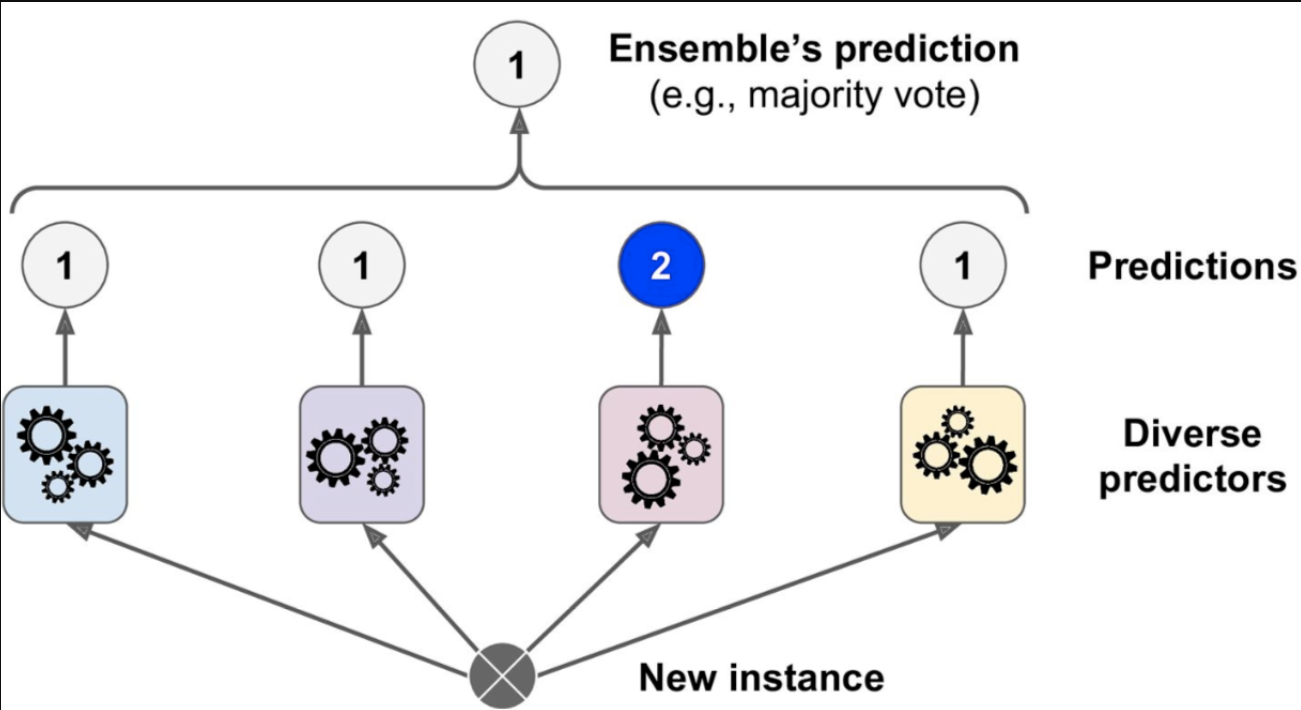
\includegraphics[width=.4\textwidth]{ensamble.png}

\subsection{Different methods}

Gabi:

There are various ways to try to solve the language recognition problem , here are some different methods that could work:

1. N-gram Language Models: N-gram language models are statistical models that estimate the probability of encountering a sequence of N consecutive words in a given language. These models capture the statistical properties of languages and can be used to compare the likelihood of a text belonging to different languages based on the observed N-grams. The language with the highest probability is considered the recognized language.

2. Machine Learning with Text Features: Machine learning algorithms can be trained on labeled datasets to learn patterns and characteristics of different languages. Features such as word frequencies, character n-grams, syntactic features, or statistical measures can be extracted from the text samples and used as input for classification algorithms like decision trees, random forests, support vector machines (SVM), or deep learning models.

3. Neural Networks with Word Embeddings: Neural network architectures, such as recurrent neural networks (RNNs) or convolutional neural networks (CNNs), can be employed for language recognition. Word embeddings, such as Word2Vec or GloVe, can be used to represent words as dense vector representations, which capture semantic and syntactic information. These embeddings can be fed into the neural network models to learn language patterns and make predictions.

 





%Gabi
\bibliographystyle{m}
\bibliography{main}

    
\end{document}
